\documentclass[10pt]{beamer}

\usetheme{metropolis}
\definecolor{WiLabRed}{RGB}{197,18,48}
\setbeamercolor{frametitle}{fg=white,bg=WiLabRed}
\setbeamercolor{progress bar}{fg=WiLabRed!90}
\setbeamercolor{title separator}{fg=WiLabRed!90}
\setbeamercolor{progress bar in section page}{fg=WiLabRed!90}
\setbeamercolor{background canvas}{bg=white}
\setbeamercolor{alerted text}{fg=WiLabRed!90}

\usepackage{appendixnumberbeamer}

\usepackage{booktabs}
\usepackage[scale=2]{ccicons}

\usepackage{pgfplots}
\usepgfplotslibrary{dateplot}

\usepackage{xspace}
\newcommand{\themename}{\textbf{\textsc{metropolis}}\xspace}

\usepackage{marvosym}
%\usepackage{subfig}
\usepackage{graphicx}\graphicspath{{images/}}
%\usepackage{subcaption}
\usepackage[framed]{./support/mcode}
\usepackage{listings}

\title{Lecture 17: Frame Synchronization Primer, Barker Sequences}
\subtitle{\textit{Software Defined Radio for Engineers} (Collins~\textit{et al.}), \textsection{8.1} \& \textsection{8.2}}
\date{}
\author{\textbf{Alexander M. Wyglinski, Ph.D.}}
\institute{ \vspace*{1in}\hfill
\includegraphics[height=1.125cm]{wilab_logo-A70916.eps} \qquad 
\includegraphics[height=1.125cm]{WPI_Inst_Prim_FulClr.eps}}
% \titlegraphic{\hfill\includegraphics[height=1.5cm]{logo.pdf}}

% Foot for all slides
\setbeamertemplate{frame footer}{\tiny \copyright~2018 by Alexander Wyglinski. This work is licensed under the Creative Commons Attribution-ShareAlike 4.0 International License. To view a copy of this license, visit http://creativecommons.org/licenses/by-sa/4.0/.}

\begin{document}

%\captionsetup[subfigure]{labelformat=empty}

%%%%%%%%%%%%%%%%%%%%%%%%%%%%%%%%%%%%%%%%%%%%%%%%%%%%%%%%%%

\maketitle




%%%%%%%%%%%%%%%%%%%%%%%%%%%%%%%%%%%%%%%%%%%%%%%%%%%%%%%%%%

\frame{

  \frametitle{Last But Not Least!}

\centering
$\downarrow$\\
Frequency Correction\\
$\downarrow$\\
Timing Recovery\\
$\downarrow$\\
Frame Synchronization\\
$\downarrow$



}



%%%%%%%%%%%%%%%%%%%%%%%%%%%%%%%%%%%%%%%%%%%%%%%%%%%%%%%%%%

\frame
{
  \frametitle{Finding the Frame}

    \begin{itemize}
        \item We have a signal corrected for any type of offsets
        \item However, the start of the frame is unknown
         \item This is simply a delay in our signal $y[n]$ 
        \begin{equation}
        \begin{split}
            u[n]=y[n-p]
        \end{split}
        \end{equation}
        
    \end{itemize}
	\hspace{5ex} where $p \in Z$

}

\frame
{
  \frametitle{Frame Structure}

    \begin{itemize}
        \item We append specifically designed preamble sequences to the frame before moduation
        \begin{figure}
  				\includegraphics[width=\linewidth]{./frame.eps}
 				 \caption{Common frame Structure of Wireless packet}
  				\label{fig:preamble followed by header and payload data}
		\end{figure}
        \item Header and payload are unknown at the receiver 
        \item However, some of the structure is still intact for decoding
    \end{itemize}

}

\frame
{
  \frametitle{Cross-Correlation}

    \begin{itemize}
        \item Consider a set of $N$ different binary sequences $b_n[m]$
        
         where $n \in [1,...,N]$ and each sequence of length $L$
         
         \item For an arbitrary binary sequence $d[m]$, we test similarity using cross-correlation 
        \begin{equation}
        \begin{split}
            C_{d,b}[k] = \sum_{m} d[m]b_n[m+k]
        \end{split}
        \end{equation}
        \item A peak will be produced at $L$th index when $d[m]=b_n[m]$
        
         ($C_{db}[m]$ will be maximized)
    \end{itemize}

}

\frame
{
  \frametitle{Barker Codes}

    \begin{itemize}
        \item Barker codes have minimum or ideal off-peak correlation
        \item Autocorrelation for a barker code $a(i)$ is given as:
        \begin{equation}
        \begin{split}
            C(k) = \sum_{i=1}^{N-k} a[i]a[i+k]
        \end{split}
        \end{equation}
        
         such that $|c[v]|\leq 1$ and $1\leq v \leq N$
    \end{itemize}

}

\frame
{
  \frametitle{Using Barker Codes}

    \begin{itemize}
        \item There are only nine known sequences for $N \in [1,2,3,4,5,7,11,13]$  
        \item The central peak is more prominent with longer sequences
        \item We typically append multiple codes together for better performance
    \end{itemize}

}

\frame
{
  \frametitle{Alternative Approach}

    \begin{itemize}
        \item We need to pad zeroes to for length equalization
        \item Data gets inflated due to this property of barker codes
        \item Applying a FIR filter may be more efficient

    \end{itemize}

}

\frame
{
  \frametitle{FIR Filter Design}

    \begin{itemize}
        \item Consider the output y of an FIR filter with taps $b_i$
        \begin{equation}
        \begin{split}
            y[n]= \sum_{i=0}^{N} b_i\cdot{u[n-i]}
        \end{split}
        \end{equation}
		 where $u[n]$ is the received signal containing signal of interest
		 \item Eq $(4)$ is identical to eq $(2)$ except for a time reversal
    \end{itemize}

}







\end{document}
